%=======================================================================
%  Biomedical Data Processing - final project (retake)
%  Written report
%=======================================================================
\documentclass[11pt,a4paper]{article}

\usepackage[utf8]{inputenc}
\usepackage[T1]{fontenc}
\usepackage[margin=2.5cm]{geometry}

% ---- typography -------------------------------------------------------
% One serif family (Charter) throughout: body text, headings and questions.
% Charter has flatter, less ornate serif terminals than a Times-based face,
% while still reading as a standard scientific text font.
\usepackage{charter}
\usepackage{courier}
\usepackage{microtype}

\usepackage{amsmath,amssymb}
\usepackage{graphicx}
\usepackage{booktabs}
\usepackage{caption}
\usepackage{subcaption}
\usepackage[hidelinks]{hyperref}
\usepackage{titlesec}
\usepackage{enumitem}

\graphicspath{{figures/}}
\setlist{itemsep=3pt,topsep=4pt,parsep=0pt}

\captionsetup{font=small,labelfont=bf,textfont=rm,width=0.92\textwidth}
\titleformat{\section}{\normalfont\large\bfseries}{\thesection}{0.8em}{}
\titleformat{\subsection}{\normalfont\bfseries}{\thesubsection}{0.8em}{}
\titleformat{\subsubsection}{\normalfont\small\bfseries}{\thesubsubsection}{0.8em}{}
\titlespacing*{\section}{0pt}{16pt}{8pt}
\titlespacing*{\subsection}{0pt}{12pt}{5pt}
\titlespacing*{\subsubsection}{0pt}{10pt}{4pt}

% Units, defined locally so the document does not depend on a particular
% siunitx version (v2 and v3 use incompatible command names).
\newcommand{\hertz}{Hz}
\newcommand{\second}{s}
\newcommand{\volt}{V}
\newcommand{\decibel}{dB}
\newcommand{\percent}{\%}
\newcommand{\milli}{m}
\newcommand{\micro}{\ensuremath{\mu}}
\newcommand{\uV}{\ensuremath{\mu}V}
\newcommand{\num}[1]{#1}
\newcommand{\SI}[2]{#1\,#2}
\newcommand{\SIrange}[3]{#1--#2\,#3}

\title{\vspace{-1.2cm}\bfseries Biomedical Data Processing:
       final project report\\[4pt]
       \large\mdseries ECG-based identification and EEG-based sleep staging}
\author{\normalsize Teodora Taleska}
\date{\normalsize August 2026}

\begin{document}
\maketitle
\thispagestyle{empty}

%=======================================================================
\section{Part I: ECG-based identification}
%=======================================================================

The aim of this part is to recover, without supervision, which of five subjects produced each
heartbeat in a single continuous ECG recording. The pipeline has six stages: R-peak detection
with Pan-Tompkins, Wiener filtering (a PQRST model as the desired signal, the inter-beat
intervals as the noise), segmentation into one-beat windows, wavelet decomposition, $K$-means
clustering into five groups, and PCA followed by re-clustering to measure the cost of the
compression. The ground-truth labels are never used inside this chain, only to score the
finished partition, and since $K$-means numbers its clusters arbitrarily, the labelling is
resolved afterwards by searching over all permutations of the five indices.

%-----------------------------------------------------------------------
\subsection{Data exploration}
\label{sec:dataexpl}
%-----------------------------------------------------------------------

The recording is a single ECG channel sampled at \SI{200}{\hertz}, \SI{605}{\second} long, 121006 samples, and contains the heartbeats of five subjects who touch the sensor in turn, one beat at a time.
Figure~\ref{fig:raw} shows a \SI{20}{\second} window of the unfiltered signal.

\begin{figure}[htbp]
  \centering
  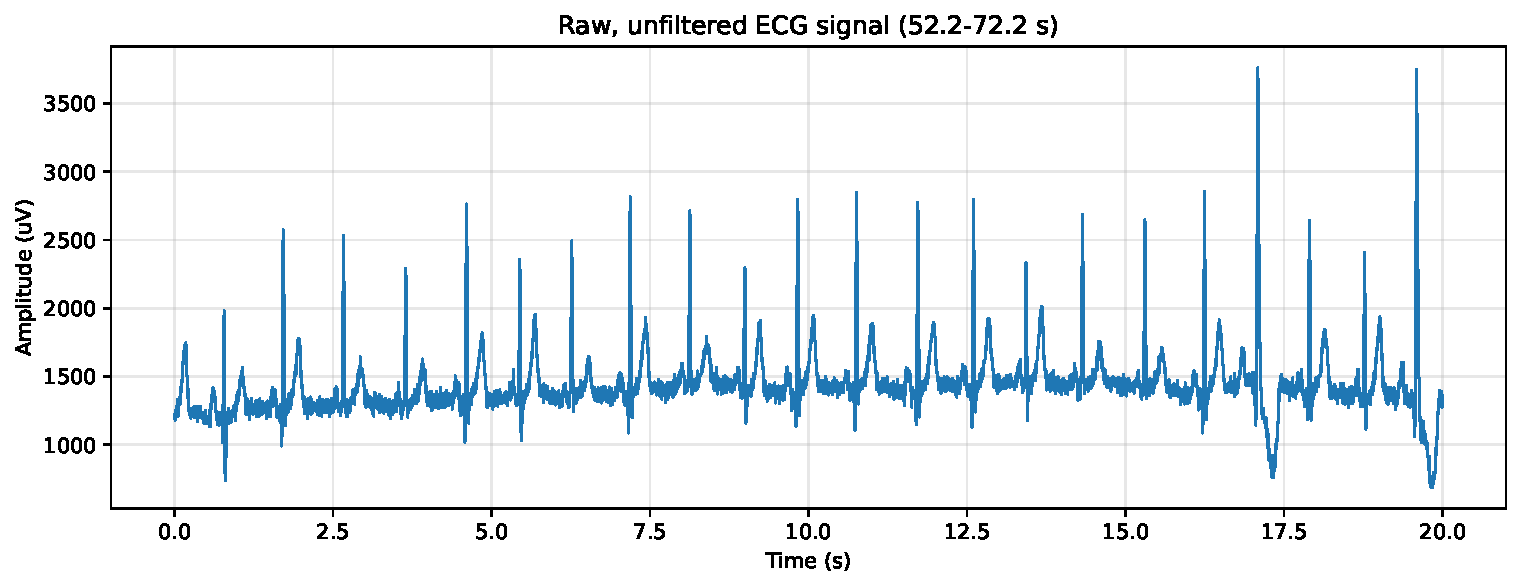
\includegraphics[width=0.95\textwidth]{p1_raw_20s.pdf}
  \caption{Twenty seconds of the raw, unfiltered ECG recording (\SIrange{52.2}{72.2}{\second}),
           with beats from several of the five subjects visible in turn.}
  \label{fig:raw}
\end{figure}
\textbf{Q: Which noise sources are present, and why?} Three sources are visible directly on this
plot.

\begin{description}[leftmargin=1.6em,style=nextline]

\item[Baseline wander.] The isoelectric line drifts slowly up and down across the window instead
of staying flat, far too slow to be cardiac activity. It tracks the electrode-skin contact,
which changes with each subject: the clearest dip in the window coincides with a change of
subject and does not have the shape of a PQRST complex.

\item[Powerline interference.] A regular ripple with a fairly constant amplitude is visible throughout the signal, including the flat segments between heartbeats where no cardiac activity is expected. Its periodic nature and consistent appearance suggest that it originates from electrical mains interference rather than the ECG itself.

\item[Broadband muscle and contact noise.] In addition to the periodic ripple, small irregular fluctuations can be observed superimposed on the ECG signal, particularly in the flatter regions between heartbeats. These non-periodic variations are consistent with muscle activity, electrode movement, or other measurement-related noise.

%\item[Powerline interference.] A regular ripple of constant amplitude is present everywhere,
%including the flat segments between beats where the heart contributes nothing. Isolated around
%\SI{50}{\hertz} it has an rms of \SI{27.9}{\uV} and a peak-to-peak amplitude of about
%\SI{104}{\uV}; its periodicity and its indifference to whether a beat is present identify it as
%mains interference rather than biology.
%
%\item[Broadband muscle and contact noise.] An irregular, burst-like fuzz sits on top of the
%ripple, best seen on the flat segments. The residual above \SI{60}{\hertz}, well outside the
%ECG band, has an rms of \SI{14.9}{\uV} and is non-periodic with intensity that varies over
%time, consistent with muscle contractions and electrode micro-movement.
\end{description}

\subsubsection{Confirmation in the frequency domain}

As an optional addition I estimated the power spectral density of the whole recording with
Welch's method (Hann window, \num{4096} samples, \SI{50}{\percent} overlap) to confirm the
three sources quantitatively. Figure~\ref{fig:rawpsd} shows the result.

\begin{figure}[htbp]
  \centering
  
\includegraphics[width=0.80\textwidth]{p1_raw_psd.pdf}
  \caption{Welch power spectral density of the complete raw recording.}
  \label{fig:rawpsd}
\end{figure}

%
%The band below \SI{0.7}{\hertz} carries \SI{22.3}{\percent} of the total power, confirming the
%baseline wander as the dominant disturbance. A narrow line stands \SI{15.1}{\decibel} above the
%floor at exactly \SI{50}{\hertz} with no line at \SI{60}{\hertz} and no harmonic at
%\SI{100}{\hertz}, confirming a clean mains tone. Above \SI{60}{\hertz}, well past where the ECG
%itself carries content, the floor stays elevated, confirming the broadband muscle and contact
%noise. The three contributions occupy fixed bands and do not change character along the record,
%so the noise is stationary, which is what justifies the single, time-invariant Wiener filter of
%Section~\ref{sec:wiener}.

\subsection{Wiener filter}
\label{sec:wiener}

The recording is cleaned with a Wiener filter built from an averaged PQRST complex as the
desired signal and the concatenated inter-beat intervals as the noise, then applied to the
whole record with weighted overlap-add filtering.

\subsubsection{Template estimation}

R-peaks are located with the Pan-Tompkins algorithm. The signal is band-pass filtered between
\SI{5}{\hertz} and \SI{11}{\hertz} using two cascaded fourth-order Butterworth stages,
differentiated with a five-point derivative, squared, and integrated with a
\SI{150}{\milli\second} moving window; peaks are then picked on this integrated signal.

\textbf{Design choices.} The assignment does not specify how to pick the peaks once the signal
is integrated, so two parameters had to be chosen. The threshold is set to exactly the mean of
the integrated signal (a factor of 1), which makes it a data-driven choice rather than a fixed
value picked by hand: between beats the integrated signal reflects only noise and stays close to
its own average, while a QRS complex produces a burst of energy well above that average, so
thresholding at the mean separates the two without needing a value tuned to this particular
recording's amplitude scale. The minimum spacing enforced between accepted peaks is set to
\SI{250}{\milli\second}, a \SI{240}{bpm} ceiling, as noted in the code comment next to it. This
sits safely above any physiologically plausible heart rate, so it can never suppress two
genuinely consecutive beats, while still being wide enough to span the \SI{150}{\milli\second}
moving-window integration, which is what stops the integrated bump from a single beat from being
picked up as two separate peaks.

\subsubsection{Creating and applying the Wiener filter}

\textbf{Q: How did you compute the Wiener filter? What methods did you use for the PSD
estimation?} The Wiener filter is designed in the frequency domain as
\[
W(f) = \frac{S_d(f)}{S_d(f) + S_n(f)},
\]
with the average PQRST complex as the model of the desired signal $d$ and the concatenated
inter-beat intervals as the model of the noise $n$.
Both signals have their mean removed before estimating their power spectral densities. The two spectra are not estimated the same way. $S_n$ is estimated with Welch's
method (Hann window, segment length equal to the filter length $L$, \SI{50}{\percent} overlap),
because the noise record is long and stationary and averaging over overlapping segments is what
keeps the variance of the estimate down. $S_d$, however, is estimated as the periodogram of the
zero-padded template rather than with Welch. This is a correction with respect to the first exam
period, where both spectra were estimated with Welch: $d$ is a single deterministic transient,
not a stationary process, so splitting it into sub-windows and averaging them, as Welch does,
mixes together shifted, non-stationary pieces of the same pulse and
broadens its spectrum. The
periodogram of the zero-padded template is the estimator that matches what $d$ actually is. The
filter's time-domain impulse response is the inverse FFT of $W(f)$, and it is applied to the
full recording with weighted overlap-add (WOLA) filtering rather than direct convolution, which
avoids having to filter \num{121\,006} samples in one block.

\textbf{Q: What length did you choose for the Wiener filter, and why?} The template is
\num{140} samples long
(\SI{0.7}{\second}). The filter length is set to $L=\num{512}$ samples (\SI{2.56}{\second}),
about \num{3.7} times the template length, which leaves enough zero-padding to resolve the
periodogram of $S_d$ at a fine frequency resolution ($\mathrm{d}f = f_s/L \approx
\SI{0.39}{\hertz}$) without truncating any of the template's spectral content. The same $L$ sets
the WOLA analysis window, so each window also spans several beats, given that Pan-Tompkins finds
\num{679} beats over the \SI{605}{\second} recording, an average rate of about \SI{67}{bpm}.
This is consistent with a filter that is designed once from global, time-invariant statistics
rather than adapted window by window.

\begin{figure}[htbp]
  \centering
  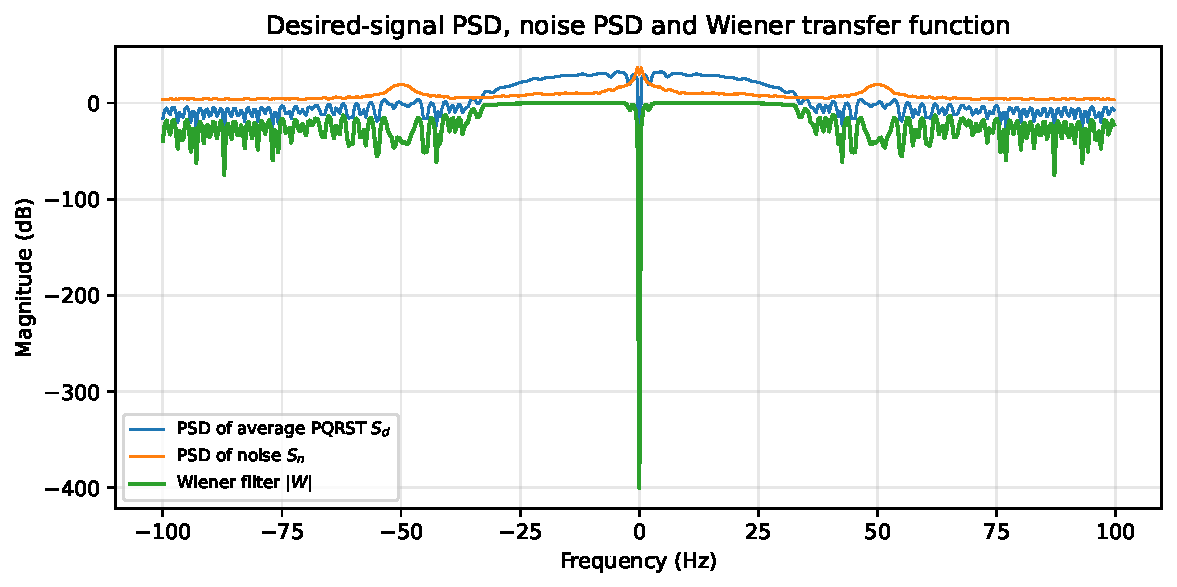
\includegraphics[width=0.8\textwidth]{p1_wiener_overview.pdf}
  \caption{PSD of the average PQRST complex ($S_d$), PSD of the noise ($S_n$), and the
           resulting Wiener filter magnitude $|W|$, all in dB.}
  \label{fig:wienerpsd}
\end{figure}

Figure~\ref{fig:wienerpsd} connects directly to the noise sources identified in
Section~\ref{sec:dataexpl}. At \SI{0}{\hertz} the filter is essentially zero: demeaning forces
$S_d(0)=0$ by construction, while $S_n(0)$ stays large because the noise segments still carry
the low-frequency baseline wander identified earlier, so the filter rejects the
near-zero-frequency band where that wander sits. In the band where the ECG carries most of its
energy, $S_d$ dominates $S_n$ and the filter stays close to unity gain, which by the definition
$W(f)=S_d/(S_d+S_n)$ can never exceed \SI{0}{\decibel}. At exactly \SI{50}{\hertz} the filter
dips sharply, matching the mains line identified before, and it rolls off further at higher
frequencies, attenuating the same broadband range where the raw PSD showed elevated muscle and
contact noise.

\textbf{Q: After filtering, recompute the R-peak locations. Do you get the same number of
R-peaks? Why (not)?}

\begin{figure}[htbp]
  \centering
  
\includegraphics[width=0.95\textwidth]{p1_rpeaks_raw_vs_filtered.pdf}
  \caption{The same \SI{20}{\second} window before and after Wiener filtering, with the
           R-peaks detected by Pan-Tompkins on each version.}
  \label{fig:rpeaks}
\end{figure}

Pan-Tompkins is re-run on the filtered signal because the detector itself depends on filtering
(its own internal band-pass and derivative stages), so a cleaner input can change which local
maxima cross the threshold. Detection gives \num{679} peaks on the raw signal and \num{676} on
the filtered one, not the same count. As an independent check, the ground-truth labels give
\num{511} uninterrupted contact runs with a median duration of \SI{0.94}{\second}; dividing each
run's duration by that median and rounding to the nearest whole number of beats (at least one)
gives an estimate of about \num{675} true heartbeats, close to both detector counts. The small
difference between the raw and filtered counts is consistent with how \texttt{wola\_filt}
behaves at the boundaries of the recording: its analysis windows overlap by design, but the
first and last windows have no neighbour to overlap with on one side, and the function
zero-pads the reconstructed signal whenever it falls short of the original length. Beats sitting
in these boundary regions are the ones most likely to be reconstructed poorly enough for
Pan-Tompkins to miss, while the interior of the recording is covered by fully overlapping
windows and filtered normally. This localised boundary behaviour of the overlap-add procedure,
rather than a general degradation of the signal, is the most likely explanation for the three
fewer peaks found after filtering.

\subsubsection{Additional questions}


\textbf{Q: Assuming independent additive noise, should you consider the average PQRST complex
as a template for the clean signal, or as a template for the signal with noise? Why?} It is a
template for the clean signal.
Under this assumption every measured beat can be written as $x_i[t] = s[t] + n_i[t]$, with
$s[t]$ the true PQRST waveform and $n_i[t]$ zero-mean noise that varies from beat to beat.
Averaging many aligned complexes cancels the noise terms while leaving the shared signal
component untouched, so the result is a noise-reduced estimate of $s[t]$, not of the noisy
signal.

\textbf{Q: Should you remove the mean from the PQRST complexes before averaging them? What
about the mean of the noise segments?} Yes, in both cases. The mean of the template carries no information about its
shape and would otherwise appear as a large DC component in $S_d$ that has nothing to do with
ECG morphology; Wiener theory also assumes zero-mean noise, so a leftover offset in the noise
segments would inflate $S_n(0)$ for reasons unrelated to the actual noise process. The effect is
directly visible in this recording: demeaning forces $S_d(0)=0$ while $S_n(0)$ stays large
because of the baseline wander identified earlier, which is exactly why the filter rejects
\SI{0}{\hertz} almost completely.

\textbf{Q: Which method and parameters did you choose to estimate the PSDs? Why?} $S_n$ is
estimated with Welch's method (Hann window, segment length $L=\num{512}$, \SI{50}{\percent}
overlap), because the noise record is long (about \SI{130}{\second}) and stationary, and
averaging over overlapping segments is what reduces the variance of the estimate; a single
periodogram of a random signal has a relative standard deviation of about \SI{100}{\percent}
regardless of record length. $S_d$ is estimated differently, as the periodogram of the
zero-padded template rather than with Welch, since $d$ is a single deterministic transient
rather than a stationary process and averaging sub-windows of it would smear its spectrum
instead of resolving it.

\textbf{Q: Do you see any edge effects after filtering? Why (not)?} A small one is plausible at
the very start and end of the recording. The \texttt{wola\_filt} function reconstructs the
filtered signal from overlapping analysis windows and explicitly zero-pads the result whenever
the reconstruction falls short of the input length; the first and last windows also lack a
neighbour to overlap with on one side. Both are boundary artefacts of the overlap-add procedure
itself, rather than of the Wiener filter's frequency response, and are the most likely
explanation for why the filtered signal yields three fewer detected R-peaks than the raw one.

%=======================================================================
\subsection{Segmentation}
%=======================================================================

The filtered signal is cut into one-beat segments around each R-peak
(\SI{0.3}{\second} before to \SI{0.4}{\second} after, as specified), and the ground-truth labels
are segmented the same way, with each segment assigned the majority label of its samples.
Averaging the segments per subject and counting how many segments each subject contributes give
the two deliverables below.

\begin{table}[htbp]
\centering
\begin{tabular}{crr}
\toprule
Subject & Count & Percentage (\%) \\
\midrule
1 & 117 & 17.31 \\
2 & 147 & 21.75 \\
3 & 40  & 5.92  \\
4 & 115 & 17.01 \\
5 & 257 & 38.02 \\
\bottomrule
\end{tabular}
\caption{Percentage of segments belonging to each subject.}
\label{tab:subjectpct}
\end{table}

The five subjects are not represented equally: subject 5 contributes the most segments and
subject 3 the fewest.

The assignment asks for the five average segments plotted separately with equally scaled axes,
which is satisfied by fixing the same $y$-limits on all five. I additionally overlaid all five
averages on one set of axes, shown in Figure~\ref{fig:avgoverlay}, since the shared axes already
make them directly comparable and a single plot makes the comparison easier to read than five
separate ones side by side.

\begin{figure}[htbp]
  \centering
  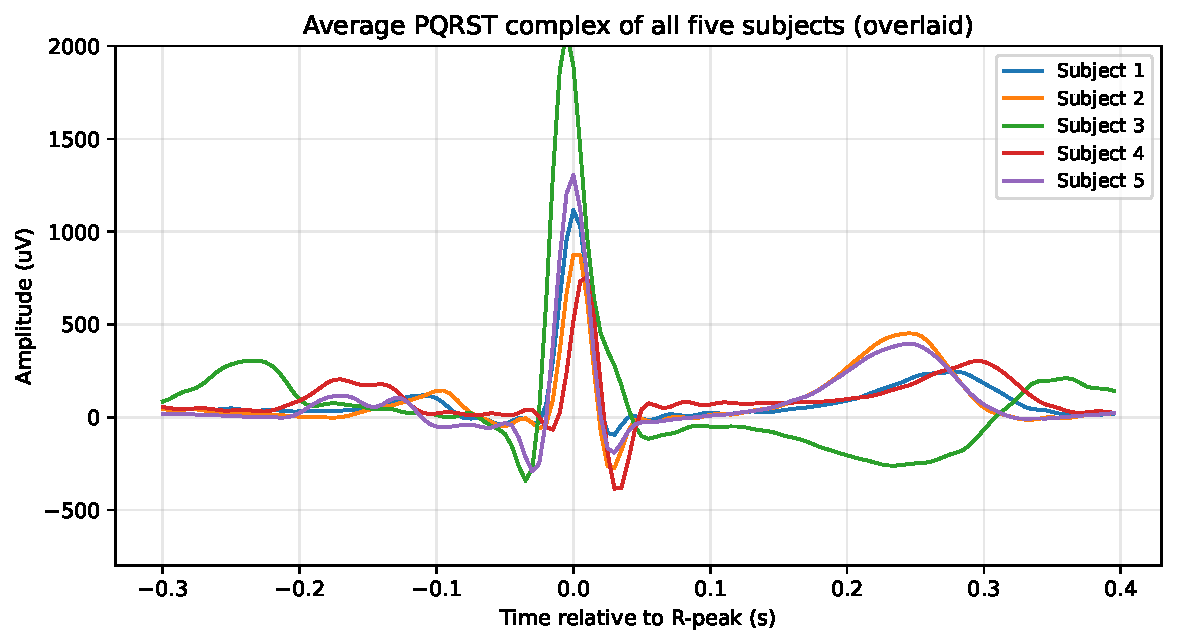
\includegraphics[width=0.85\textwidth]{p1_avg_subjects_overlay.pdf}
  \caption{Average PQRST complex of all five subjects, overlaid on shared axes.}
  \label{fig:avgoverlay}
\end{figure}

Subject 3 stands out from the other four: its R-peak is noticeably higher, and where the other
subjects settle into a positive bump after the R-peak, subject 3's average stays negative over
that same stretch. This lines up with the assignment's own background on the data, which states
that subject 3, unlike the other four, has valvular heart disease, a condition that affects how
the heart's chambers fill and contract and would be expected to change the shape of the
electrical signal relative to a healthy beat.

\subsubsection{Additional questions}

\textbf{Q: Do you see any defining differences between the average PQRST complex of each
subject?} Yes. All five averages share the same overall structure and are aligned at the
R-peak, but they differ in QRS amplitude, width and the morphology of the surrounding waves.
Subject 3 is the clearest case: besides the taller R-peak, its average complex stays negative
where the others show a positive wave, consistent with the valvular heart disease noted for
that subject in the assignment description. The remaining four subjects vary more moderately
among themselves in amplitude and width, without such a qualitative change in shape.

%=======================================================================
\subsection{Wavelet decomposition}
%=======================================================================

Each \SI{0.7}{\second} segment is decomposed with a level-5 Daubechies-4 (db4) wavelet
transform, giving six coefficient arrays per segment (cA5 through cD1, \num{11}+\num{11}+
\num{15}+\num{23}+\num{40}+\num{73}=\num{173} values in total), concatenated into one
\num{173}-value feature vector per beat. It is this feature vector, not the raw \num{140}-sample
segment, that is used as input to the clustering algorithm in the next section.

\textbf{Q: Select two wavelet coefficients that you consider most important. Visualize them in
a two-dimensional space, coloured by ground-truth label.} Importance is measured as variance
across the \num{676} segments, after first discarding coefficients whose variance is
effectively zero (a \texttt{VarianceThreshold} step): those carry no information regardless of
how the ranking is done, so they are removed before ranking rather than left to compete with
genuinely informative coefficients. Among what remains, the two with the highest variance are
kept: \texttt{cA5[8]} and \texttt{cA5[10]}, both from the coarsest approximation band rather
than from any detail band. That is not a coincidence: \texttt{cA5} describes the broad shape
and amplitude of the whole beat, and it is at that scale, not in the fast, fine detail, that the
subjects differ most, matching Section~1.3's finding that subject 3's average complex differs
from the others mainly in overall amplitude and shape.

Plotted in this space (Figure~\ref{fig:kmeans2d} in Section~1.5, left panel), subject 3 is
clearly separated from the other four along this pair of coordinates. The remaining four
subjects overlap substantially with each other, which is expected from the selection method:
ranking by variance alone favours whichever coefficients vary the most across the whole
dataset, and that is driven by the subject that differs most overall (subject 3), without any
guarantee that the other four are pulled apart from one another too.

\subsubsection{Additional questions}

\textbf{Q: What is the advantage of this wavelet decomposition before clustering, compared to
simply clustering the ECG segments directly?} The decomposition does not shrink the number of
values, \num{173} coefficients from a \num{140}-sample segment is not a smaller representation,
but it separates the beat into components at different scales instead of leaving it as a flat
sequence of raw time samples. That separation is what the coefficient-selection step above
relies on: the two coefficients that best set subject 3 apart both turned out to sit in the
coarsest band, the one describing overall shape and amplitude, while the fine-detail bands
contribute comparatively little to that particular difference. Clustering directly on raw
samples has no equivalent way to tell a broad shape difference apart from fine timing jitter,
since both simply show up as a pointwise difference at some sample index; the wavelet
decomposition keeps that distinction explicit and available to work with.

%=======================================================================
\subsection{$K$-means clustering}
%=======================================================================

$K$-means with $k=5$ is fit on the same two coefficients selected in Section~1.4
(\texttt{cA5[8]} and \texttt{cA5[10]}, z-scored first), and \texttt{match\_labels} permutes the
resulting cluster indices to whichever assignment best agrees with the ground-truth subjects,
since $K$-means itself has no notion of which cluster index corresponds to which subject.

\begin{figure}[htbp]
  \centering
  \begin{subfigure}{0.48\textwidth}
    \centering
    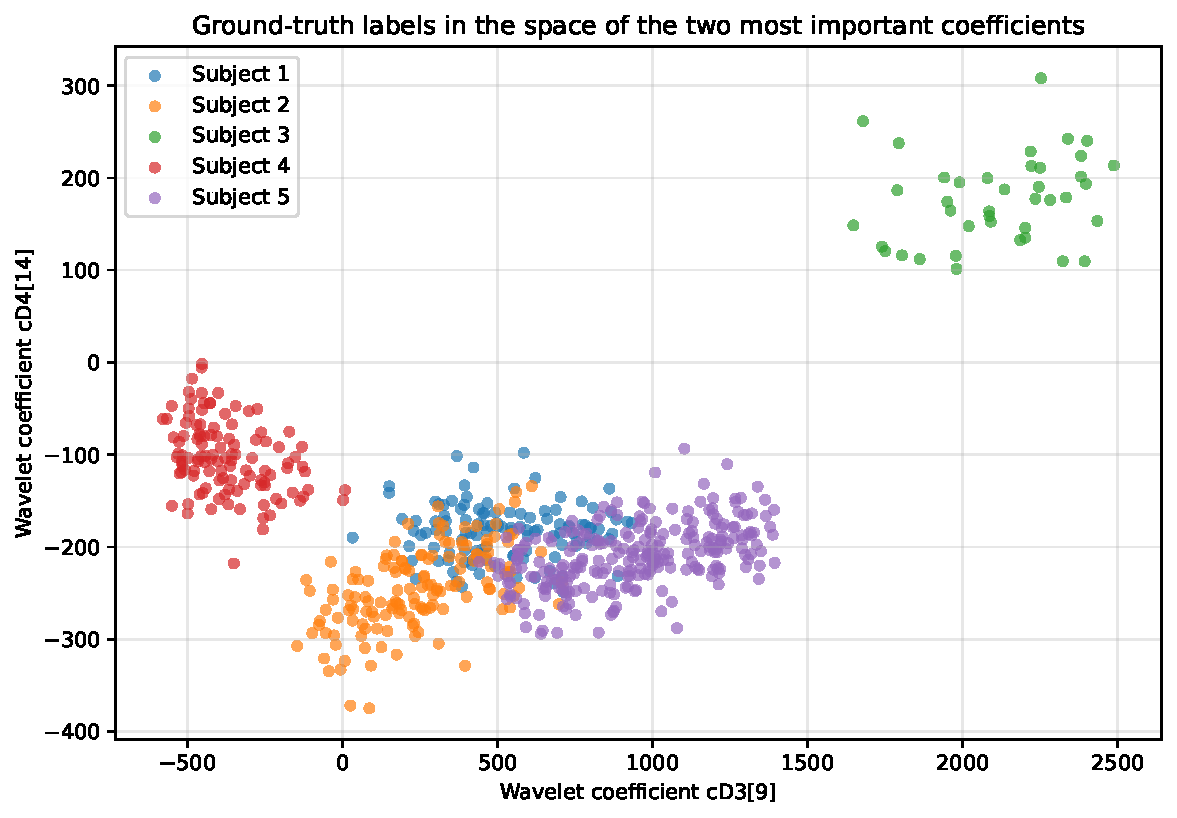
\includegraphics[width=\textwidth]{p1_wavelet_groundtruth_2d.pdf}
    \caption{Ground-truth labels (Section 1.4)}
  \end{subfigure}
  \hfill
  \begin{subfigure}{0.48\textwidth}
    \centering
    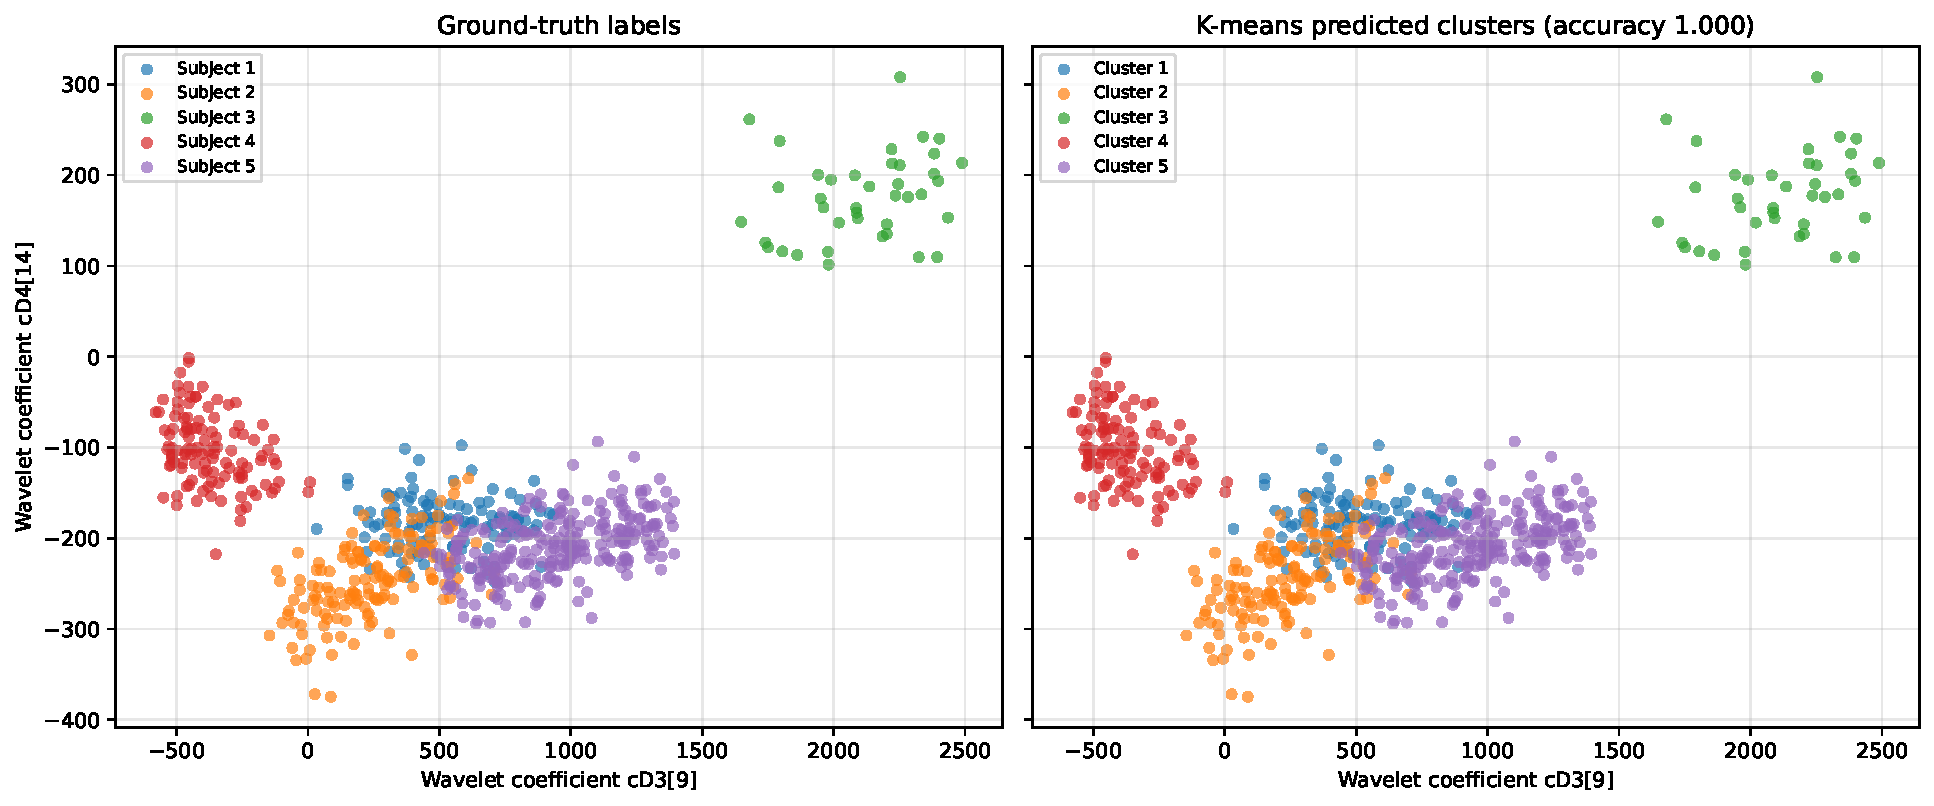
\includegraphics[width=\textwidth]{p1_kmeans_wavelet_2d.pdf}
    \caption{$K$-means clusters, matched to ground truth}
  \end{subfigure}
  \caption{Ground-truth labels versus $K$-means clusters in the space of the same two
           coefficients, \texttt{cA5[8]} and \texttt{cA5[10]}.}
  \label{fig:kmeans2d}
\end{figure}

Accuracy after matching is \num{0.420}; the confusion matrix is shown alongside the
post-reduction one for comparison in Section~1.6. Subject 3 is recovered
almost perfectly, \num{38} of its \num{40} segments are correctly assigned, matching
Figure~\ref{fig:kmeans2d}, where the green cluster sits apart from the rest. Subjects 1, 2 and 5
are the opposite case: their rows are spread across several columns rather than concentrated on
the diagonal, because in this two-coefficient space they occupy the same overlapping region
(visible already in the ground-truth panel). $K$-means still partitions that region into three
clusters, since it always assigns every point to its nearest centroid regardless of whether the
underlying classes are actually separable there, so the boundaries it draws through the overlap
are essentially arbitrary with respect to the true subject identity.

\textbf{Q: Did you normalise the wavelet coefficients before classification (without
dimensionality reduction)?} Yes. Both coefficients are z-scored with \texttt{StandardScaler}
before $K$-means is fit, so that neither one dominates the Euclidean distance purely because of
its numerical range. In this particular pair the two coefficients' variances, \num{711700.64}
for \texttt{cA5[8]} and \num{516391.97} for \texttt{cA5[10]} (Section 1.4), are already the same
order of magnitude, so normalisation mainly enforces the general principle here rather than
correcting a large scale mismatch; it is applied regardless, since relying on the two selected
coefficients happening to be on comparable scales would not generalise to a different pair.

\subsubsection{Additional questions}

\textbf{Q: Is the result of the unsupervised clustering always the same? Why (not)?} Not in
general. $K$-means starts from randomly initialised centroids, and different initialisations
can converge to different local minima, particularly where classes overlap as they do here for
subjects 1, 2 and 5. In this notebook the result is reproducible from run to run only because
\texttt{random\_state=42} fixes that randomness; without a fixed seed, the exact cluster
boundaries through the overlapping region could come out differently each time, even though the
well-separated subject 3 cluster would likely be recovered consistently regardless.

\textbf{Q: Why do the names of the cluster labels not always match the names of the class
labels?} $K$-means has no access to the ground-truth labels and numbers its clusters
arbitrarily, in whatever order it happens to initialise or converge. Cluster ``1'' has no reason
to correspond to subject 1. \texttt{match\_labels} searches over all permutations of the five
indices and keeps whichever relabelling maximises agreement with the ground truth, which is
what makes the accuracy and confusion matrix above meaningful.

\textbf{Q: Is it a good idea to normalise the wavelets before classification? Why (not)?} Yes,
as a general rule, since $K$-means clusters purely by Euclidean distance, a coefficient with a
larger numerical range would automatically carry more weight in that distance than a more
informative coefficient on a smaller scale, for reasons that have nothing to do with which one
actually separates the subjects.

\textbf{Q: How do you decide which wavelet values are the most relevant to model the ECG
segments? Why?} As in Section~1.4, relevance is measured as variance across the \num{676}
segments after discarding near-constant coefficients, and the two coefficients kept here are
the same highest-variance pair found there, \texttt{cA5[8]} and \texttt{cA5[10]}, both from the
coarsest approximation band, since that is the scale at which the subjects differ most in
overall shape and amplitude.

%=======================================================================
\subsection{Dimensionality reduction}
%=======================================================================

The wavelet features are reduced with PCA, fit on the full \num{173}-coefficient set
\texttt{X\_wav} (shape \num{676}$\times$\num{173}) after z-scoring it with
\texttt{StandardScaler}, the same order (normalise first, then reduce) as motivated in
Section~1.4: PCA looks for directions of maximum variance, so without normalising first it
would be dominated by whichever coefficients happen to have the largest raw scale, the coarse
approximation band again, rather than by whichever directions are actually most informative.
The number of components is chosen as the smallest number that reaches \SI{90}{\percent}
cumulative explained variance, a standard, simple stopping rule that does not require deciding
on a target dimensionality by hand; on this dataset that threshold is reached at $N=\num{40}$
components, a real reduction from \num{173} but far more than the \num{2} coefficients used in
Section~1.5. For the 2D visualisation, the two dimensions plotted are the first two principal
components, \texttt{PC1} and \texttt{PC2}: PCA already orders its components by variance, so
these are ``the two most relevant dimensions'' under the same variance criterion used throughout
this part, with no separate selection step needed.

\begin{table}[htbp]
\centering
\begin{minipage}{0.48\textwidth}
\centering
\textbf{Before reduction} \\[2pt]
$\begin{pmatrix}
66 & 13 & 0 & 19 & 19 \\
16 & 41 & 0 & 23 & 67 \\
1 & 0 & 38 & 1 & 0 \\
57 & 19 & 0 & 20 & 19 \\
44 & 58 & 0 & 36 & 119
\end{pmatrix}$
\end{minipage}
\hfill
\begin{minipage}{0.48\textwidth}
\centering
\textbf{After reduction (PCA, $N=40$)} \\[2pt]
$\begin{pmatrix}
117 & 0 & 0 & 0 & 0 \\
0 & 147 & 0 & 0 & 0 \\
0 & 0 & 40 & 0 & 0 \\
0 & 0 & 0 & 115 & 0 \\
0 & 0 & 0 & 0 & 257
\end{pmatrix}$
\end{minipage}
\caption{Confusion matrices before and after dimensionality reduction.}
\label{tab:cmcompare}
\end{table}

Accuracy rises from \num{0.420118} before dimensionality reduction to \num{1.000000} after it
with PCA, even though this step is nominally a \emph{reduction}, because what is being compared
is not ``more dimensions vs.\ fewer'' but
``\num{2} manually picked raw coefficients vs.\ \num{40} dimensions distilled from the entire
\num{173}-coefficient representation'': the PCA step still uses far more of the original
information than the two-coefficient visualisation in Section~1.5 ever did, the ``reduction'' is
only relative to the full \num{173}, not to the \num{2} used before.

\textbf{Q: How did you reduce the feature dimensionality as much as possible? Did you use any
normalisation? If yes, when?} As described above: PCA on the full \num{173}-value wavelet
feature vector, keeping the smallest number of components that explains at least
\SI{90}{\percent} of the variance ($N=\num{40}$), with the \texttt{StandardScaler} normalisation
applied before PCA, not after.

\subsubsection{Additional questions}

\textbf{Q: Should you normalise before dimensionality reduction? What about after
dimensionality reduction?} Yes before: PCA is sensitive to feature scale and would otherwise be
dominated by whichever raw coefficients have the largest numerical range, not necessarily the
most informative ones. Not after: PCA already orders the kept components by how much variance
they explain on the normalised input, so re-normalising afterwards would force components that
are not equally informative to contribute equally to any distance computed on them, undoing
that ordering rather than preserving it.

\end{document}
